The development of plane finite elements is elaborated with the assistance of the relatively simply
generated four-noded bilinear Lagrange element and specified for the case of a rectangular
element.
\subsection{Shape Functions}
The shape function of element node one can be derived by multiplication of the one-dimensional
Lagrange polynomials $N_1^1 (\xi_1 )$ and $N_2^1 (\xi_2 )$ corresponding to this node, which are expressed
in the natural coordinate directions $\xi_1$ or $ \xi_2$ .
\begin{equation}
\label{eqn:3.33}
 N_{1}^{1}\left(\xi_{1}\right)=\frac{1}{2}\left(1-\xi_{1}\right) \quad N_{2}^{1}\left(\xi_{2}\right)=\frac{1}{2}\left(1-\xi_{2}\right) 
\end{equation}
Multiplication of $N_1^1(\xi_1)$ and $N_2^1(\xi_2)$ yields the shape function $N^1(\xi_ 1 , \xi_ 2 )$ for node one. The natural coordinates $\xi_ 1$ and $\xi_ 2$ are assembled in the vector $\xi_ = [\xi_ 1 \xi_ 2 ]$ T in order to show the dependencies.
\begin{equation}
\label{eqn:3.34}
    \label{eqn:334}
    \begin{split}
        {N^1}\left( {{\xi _1},{\xi _2}} \right) &= {N^1}(\xi ) = N_1^1\left( {{\xi _1}} \right)N_2^1\left( {{\xi _2}} \right) \\ &= \frac{1}{2}\left( {1 - {\xi _1}} \right)\frac{1}{2}\left( {1 - {\xi _2}} \right) = \frac{1}{4}\left( {1 - {\xi _1}} \right)\left( {1 - {\xi _2}} \right) \\ &= \frac{1}{4}\left( {1 - {\xi _1} - {\xi _2} + {\xi _1}{\xi _2}} \right)
    \end{split}
\end{equation}
As we can conclude from equation (\ref{eqn:334}), the shape function $N^1(\xi)$ contains constant, linear as
well as bilinear segments. In figure \ref{fig:3.6}, these segments correspond to the square in the Pascal
triangle characterised by $p = 1$. As a preliminary observation to the oncoming explanation of
approximating continuous variables, it may be noted that a two-dimensional polynomial of
plane elements is formed with the sum of all shape functions $N^i(\xi)$ that have the corresponding
weights. The shape functions of the element nodes two to four can be generated in an analogous way.
\begin{equation}
\label{eqn:3.35}
    \begin{gathered}
{N^1}(\xi ) = \frac{1}{4}\left( {1 - {\xi _1}} \right)\left( {1 - {\xi _2}} \right)\\
{N^2}(\xi ) = \frac{1}{4}\left( {1 + {\xi _1}} \right)\left( {1 - {\xi _2}} \right)\\
{N^3}(\xi ) = \frac{1}{4}\left( {1 + {\xi _1}} \right)\left( {1 + {\xi _2}} \right)\\
{N^4}(\xi ) = \frac{1}{4}\left( {1 - {\xi _1}} \right)\left( {1 + {\xi _2}} \right)
\end{gathered}
\end{equation}

Furthermore, in order to approximate the strains and to generate the Jacobi matrix, derivations
of shape functions with respect to the natural coordinates $\xi_ 1$ and $\xi_ 2$ are required. These can
be found as follows:
\[\arraycolsep=10pt\def\arraystretch{3.2}
\begin{equation}
\label{eqn:3.36}
\begin{array}{cccc}
{\dfrac{{\partial {N^1}({\boldsymbol{\xi }})}}{{\partial {\xi _1}}} = N_{;1}^1({\boldsymbol{\xi }}) =  - \dfrac{1}{4}\left( {1 - {\xi _2}} \right)}&{\dfrac{{\partial {N^1}({\boldsymbol{\xi }})}}{{\partial {\xi _2}}} = N_{;2}^1({\boldsymbol{\xi }}) =  - \dfrac{1}{4}\left( {1 - {\xi _1}} \right)}\\
{\dfrac{{\partial {N^2}({\boldsymbol{\xi }})}}{{\partial {\xi _1}}} = N_{;1}^2({\boldsymbol{\xi }}) = \dfrac{1}{4}\left( {1 - {\xi _2}} \right)}&{\dfrac{{\partial {N^2}({\boldsymbol{\xi }})}}{{\partial {\xi _2}}} = N_{;2}^2({\boldsymbol{\xi }}) =  - \dfrac{1}{4}\left( {1 + {\xi _1}} \right)}\\
{\dfrac{{\partial {N^3}({\boldsymbol{\xi }})}}{{\partial {\xi _1}}} = N_{;1}^3({\boldsymbol{\xi }}) = \dfrac{1}{4}\left( {1 + {\xi _2}} \right)}&{\dfrac{{\partial {N^3}({\boldsymbol{\xi }})}}{{\partial {\xi _2}}} = N_{;2}^3({\boldsymbol{\xi }}) = \dfrac{1}{4}\left( {1 + {\xi _1}} \right)}\\
{\dfrac{{\partial {N^4}({\boldsymbol{\xi }})}}{{\partial {\xi _1}}} = N_{;1}^4({\boldsymbol{\xi }}) =  - \dfrac{1}{4}\left( {1 + {\xi _2}} \right)}&{\dfrac{{\partial {N^4}({\boldsymbol{\xi }})}}{{\partial {\xi _2}}} = N_{i2}^4({\boldsymbol{\xi }}) = \dfrac{1}{4}\left( {1 - {\xi _1}} \right)}
\end{array}
\end{equation}
%---------------------------------------------------------
\subsection{Geometry}
The geometry of a four-noded Lagrange element in physical and natural space is shown in figure
\ref{fig:geometry}. An arbitrary material point within the quadrangular element is unequivocally identifiable
by its physical and natural coordinates.
\begin{equation}
 \boldsymbol{X}=\left[\begin{array}{lll}X_{1} & X_{2}\end{array}\right]^{T} \qquad \boldsymbol{\xi}=\left[\begin{array}{ll}\xi_{1} & \xi_{2}\end{array}\right]^{T} 
\end{equation}

Positions of the corner nodes are assembled in the element position vector.
\begin{equation}
    \begin{align}
{X^e} &= {\left[ {\begin{array}{*{20}{c}}
{X_1^{e1}}&{X_2^{e1}}&{X_1^{e2}}&{X_2^{e2}}&{X_1^{e3}}&{X_2^{e3}}&{X_1^{e4}}&{X_2^{e4}}
\end{array}} \right]^T}\\
&= {\left[ {\begin{array}{*{20}{c}}
{{X^e}^{1T}}&{{X^{e2}}^T}&{{X^{e3T}}}&{{X^{e4T}}}
\end{array}} \right]^T}
\end{align}
\end{equation}

Within the scope of isoparametric approximation of geometry and element variables, the continuous position vector $\boldsymbol{X}$ is described with the help of shape functions $N^i(\boldsymbol{\xi})$ in natural coordinates and with the help of discrete positions of element node $\boldsymbol{X}^e}$.

\begin{figure}
    \centering
    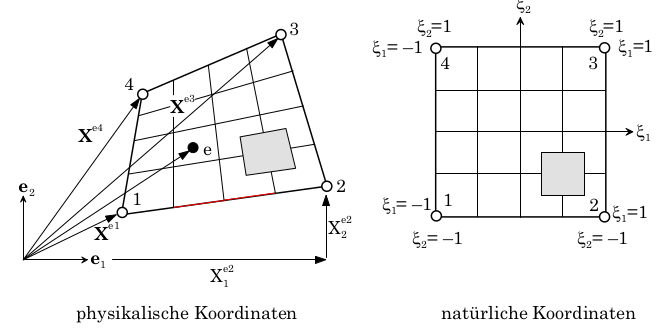
\includegraphics[scale=0.5]{Figure2/Chap2/Bilinear element.png}
    \caption{Bilinear element in physical and natural coordinates}
    \label{fig:geometry}
\end{figure}
\begin{equation}
\label{eqn:339}
 \boldsymbol{X}\left(\xi_{1}, \xi_{2}\right)=\boldsymbol{X}(\boldsymbol{\xi}) \approx \tilde{\boldsymbol{X}}(\boldsymbol{\xi})=\sum_{i=1}^{N \mathrm{~N}} \boldsymbol{X}^{e i} N^{i}(\boldsymbol{\xi})=\sum_{i=1}^{4} \boldsymbol{X}^{e i} N^{i}(\boldsymbol{\xi}) 
\end{equation}
where $NN$ generally stands for the number of element nodes. Alternatively, the continuous
position vector can be approximated by means of the shape function matrix $N(\boldsymbol{\xi})$ and with the
element position vector $\boldsymbol{X}^e$.
\vspace{0.1cm}
\begin{equation}
\small
\underbrace{\left[\begin{array}{c}
\tilde{X}_{1}(\xi) \\
\tilde{X}_{2}(\xi)
\end{array}\right]}_{\bar{X}(\xi)}=\underbrace{\left[\begin{array}{cccccccc}
N^{1}(\xi) & 0 & N^{2}(\xi) & 0 & N^{3}(\xi) & 0 & N^{4}(\xi) & 0 \\
0 & N^{1}(\xi) & 0 & N^{2}(\xi) & 0 & N^{3}(\xi) & 0 & N^{4}(\xi)
\end{array}\right]}_{N(\xi)} \underbrace{\left[\begin{array}{c}
X_{1}^{e 1} \\
X_{2}^{e 1} \\
X_{1}^{e 2} \\
X_{2}^{e 2} \\
X_{1}^{e 3} \\
X_{2}^{e 3} \\
X_{1}^{e 4} \\
X_{2}^{e 4}
\end{array}\right]}_{X^{e}}
\label{eqn:340}
\end{equation}

Equation (\ref{eqn:340}) describes the approximation of physical coordinates as function of natural
coordinates ($NN = 4$)
\begin{equation}
\label{eqn:341}
 \tilde{\boldsymbol{X}}(\boldsymbol{\xi})=\mathbf{N}(\boldsymbol{\xi}) \boldsymbol{X}^{e} \qquad \qquad \boldsymbol{X}^{e}=\left[\begin{array}{lllll}X_{1}^{e 1} & X_{2}^{e 1} & \cdots & X_{1}^{e N N} & X_{2}^{e N N}
\end{array}\right]^{T} 
\end{equation}
by means of shape function matrix $N(\boldsymbol{\xi})$, which is made up of diagonal matrices of shape
functions $N i (\boldsymbol{\xi})$ that correspond to element nodes $i$.
\begin{equation}
\label{eqn:3.42}
 \mathbf{N}^{i}(\boldsymbol{\xi})=\left[\begin{array}{cc}N^{i}(\boldsymbol{\xi}) & 0 \\ 0 & N^{i}(\boldsymbol{\xi})\end{array}\right] \qquad \qquad \mathbf{N}=\left[\begin{array}{lll}\mathbf{N}^{1} & \cdots & \mathbf{N}^{N N}\end{array}\right], NN=4 
\end{equation}

The mapping from natural to physical coordinates according to equations (\ref{eqn:339}) to (\ref{eqn:341}) can be generally described by the functional relation,
\begin{equation}
\label{eqn:3.43}
 \boldsymbol{X}=\boldsymbol{X}(\boldsymbol{\xi}) \qquad \qquad \qquad X_{\beta}=X_{\beta}(\boldsymbol{\xi}), \quad \beta=1,2 
\end{equation}
where the ’Tilda’ approximation designation is omitted. The inverse mapping describes the natural coordinates as function of the physical coordinates.
\begin{equation}
 \boldsymbol{\xi}=\boldsymbol{\xi}(\boldsymbol{X}) \qquad \qquad \qquad \xi_{\alpha}=\xi_{\alpha}(\boldsymbol{X}), \quad \alpha=1,2 
 \label{eqn:3.44}
\end{equation}
\subsection{Jacobi Transformation}
\begin{figure}
    \centering
    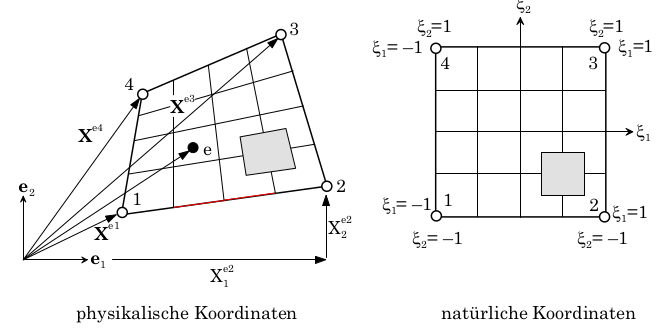
\includegraphics[scale=0.5]{Figure2/Chap2/Bilinear element.png}
    \caption{Jacobi transformation of a surface element $dA$ in natural coordinates}
    \label{fig:3.10}
\end{figure}
The calculation of the strain vector $\varepsilon$ according to equation (\ref{eqn:3.12}) requires that the displacement
components be derivated with respect to physical coordinates X. Since displacement components
as well as approximation of the position vector within the scope of the isoparametric element
concept are expressed as functions of natural coordinates, the necessary derivations with respect
to physical coordinates must be obtained indirectly over the partial derivatives of equation
(\ref{eqn:3.44}). Applying the chain rule to equation (\ref{eqn:3.44}) results in the transformation relation between derivatives with respect to physical and natural coordinates, respectively.
\begin{equation}
\label{eqn:3.45}
 \frac{\partial}{\partial \xi_{\alpha}}=\frac{\partial}{\partial X_{1}} \frac{\partial X_{1}}{\partial \xi_{\alpha}}+\frac{\partial}{\partial X_{2}} \frac{\partial X_{2}}{\partial \xi_{\alpha}}=\frac{\partial}{\partial X_{\beta}} \frac{\partial X_{\beta}}{\partial \xi_{\alpha}} 
\end{equation}

This equation can alternatively be given in the matrix form with the help of the Jacobi matrix $\boldsymbol{J(\xi)}$.
\begin{equation}

 \left[\begin{array}{c}\frac{\partial}{\partial \xi_{1}} \\ \frac{\partial}{\partial \xi_{2}}\end{array}\right]=\left[\begin{array}{ll}\frac{\partial X_{1}}{\partial \xi_{1}} & \frac{\partial X_{2}}{\partial \xi_{1}} \\ \frac{\partial X_{1}}{\partial \xi_{2}} & \frac{\partial X_{2}}{\partial \xi_{2}}\end{array}\right]\left[\begin{array}{c}\frac{\partial}{\partial X_{1}} \\ \frac{\partial}{\partial X_{2}}\end{array}\right] \qquad  \qquad \frac{\partial}{\partial \xi}=\mathbf{J}(\xi) \frac{\partial}{\partial \boldsymbol{X}} 
 \label{eqn:3.46}
\end{equation}

The rule for derivating functions in natural coordinates with respect to physical coordinates is
obtainable by inversion of equation (\ref{eqn:3.46}) with ${\rm{|J(}}\xi {\rm{)|  >  0}}{\rm{.}}$.
\begin{equation}
\label{eqn:3.47}
 \frac{\partial}{\partial \boldsymbol{X}}=\mathbf{J}^{-1}(\boldsymbol{\xi}) \frac{\partial}{\partial \boldsymbol{\xi}} 
\end{equation}
The inverse Jacobi matrix $J_{−1}(\xi)$ needed for this can be obtained directly by inverting the
$2 x 2 $ Jacobi matrix $J(\xi)$
\begin{equation}
\label{eqn:3.48}
 \mathbf{J}^{-1}(\boldsymbol{\xi})=\frac{1}{|\mathbf{J}(\boldsymbol{\xi})|}\left[\begin{array}{cc}\frac{\partial X_{2}}{\partial \xi_{2}} & -\frac{\partial X_{2}}{\partial \xi_{1}} \\ -\frac{\partial X_{1}}{\partial \xi_{2}} & \frac{\partial X_{1}}{\partial \xi_{1}}\end{array}\right] 
\end{equation}
where the Jacobi determinant is given by the expression
\begin{equation}
\label{eqn:3.49}
 |\mathbf{J}|=\frac{\partial X_{1}}{\partial \xi_{1}} \frac{\partial X_{2}}{\partial \xi_{2}}-\frac{\partial X_{1}}{\partial \xi_{2}} \frac{\partial X_{2}}{\partial \xi_{1}} 
\end{equation}
and the derivatives of physical coordinates are obtainable with respect to natural coordinates
from the approximation of the position vector $X = [X_1 X_2 ]^T $according to equations (\ref{eqn:339}) or (\ref{eqn:341}).
\begin{equation}
\label{eqn:3.50}
 \frac{\partial X_{\beta}(\boldsymbol{\xi})}{\partial \xi_{\alpha}}=\sum_{i=1}^{N} X_{\beta}^{e i} N_{; \alpha}^{i}(\boldsymbol{\xi}) \qquad \qquad \frac{\partial \boldsymbol{X}(\boldsymbol{\xi})}{\partial \xi_{\alpha}}=\boldsymbol{X}_{; \alpha}(\boldsymbol{\xi})=\mathbf{N}_{; \alpha}(\boldsymbol{\xi}) \boldsymbol{X}^{e} 
\end{equation}

Formally, we can get the inverse of the Jacobi matrix by applying the chain rule to functional
relation \( X_{\beta}=X_{\beta}(\boldsymbol{\xi}) \) given in equation (\ref{eqn:3.43})
\begin{equation}
\label{eqn:3.51}
 \frac{\partial}{\partial X_{\beta}}=\frac{\partial}{\partial \xi_{1}} \frac{\partial \xi_{1}}{\partial X_{\beta}}+\frac{\partial}{\partial \xi_{2}} \frac{\partial \xi_{2}}{\partial X_{\beta}}=\frac{\partial}{\partial \xi_{\alpha}} \frac{\partial \xi_{\alpha}}{\partial X_{\beta}} 
\end{equation}

Definition of the Jacobi matrix:
\begin{equation}
\label{eqn:3.52}
 \left[\begin{array}{c}\frac{\partial}{\partial X_{1}} \\ \frac{\partial}{\partial X_{2}}\end{array}\right]=\left[\begin{array}{cc}\frac{\partial \xi_{1}}{\partial X_{1}} & \frac{\partial \xi_{2}}{\partial X_{1}} \\ \frac{\partial \xi_{1}}{\partial X_{2}} & \frac{\partial \xi_{2}}{\partial X_{2}}\end{array}\right]\left[\begin{array}{c}\frac{\partial}{\partial \xi_{1}} \\ \frac{\partial}{\partial \xi_{2}}\end{array}\right]
 \qquad \qquad \frac{\partial}{\partial \boldsymbol{X}}=\mathbf{J}^{-1}(\xi) \frac{\partial}{\partial \xi} 
\end{equation}

By means of coefficient comparison of the inverse Jacobi matrix according to equations (\ref{eqn:3.48})
and (\ref{eqn:3.52}), we can get the identities
\begin{equation}
\label{eqn:3.53}
 \begin{aligned} \frac{\partial \xi_{1}}{\partial X_{1}} &=\frac{1}{|\mathbf{J}(\boldsymbol{\xi})|} \frac{\partial X_{2}}{\partial \xi_{2}} & \frac{\partial \xi_{2}}{\partial X_{1}} &=-\frac{1}{|\mathbf{J}(\boldsymbol{\xi})|} \frac{\partial X_{2}}{\partial \xi_{1}} \\ \frac{\partial \xi_{1}}{\partial X_{2}} &=-\frac{1}{|\mathbf{J}(\boldsymbol{\xi})|} \frac{\partial X_{1}}{\partial \xi_{2}} & \frac{\partial \xi_{2}}{\partial X_{2}} &=\frac{1}{|\mathbf{J}(\boldsymbol{\xi})|} \frac{\partial X_{1}}{\partial \xi_{1}} \end{aligned} 
\end{equation}

A transformation relation of the surface element $dA$ can be generated from the first of these
identities in physical and natural coordinates.
\begin{equation}
\label{eqn:3.54}
 d A=d X_{1} d X_{2}=|\mathbf{J}(\boldsymbol{\xi})| d \xi_{1} d \xi_{2} 
\end{equation}
Alternatively, we can derive these transformation relations that are presented in figure 3.10 with
assistance of surface elements, in physical and natural coordinates. For that purpose, vectors
$dX_ 1 , dX_ 2 , d\xi_1 $ and $d\xi$ 2 spanning the surface elements are defined. The surface elements are
given with the help of these definitions by the magnitude of the vector product of vectors $dX_ 1$
and $dX_ 2$ that is $d\xi_1$ and $d\xi_2$ .
\begin{equation}
\label{eqn:3.55}
 \begin{aligned} d A &=\left|d \boldsymbol{X}_{1} \times d \boldsymbol{X}_{2}\right| =\sin \alpha\left|d \boldsymbol{X}_{1}\right|\left|d \boldsymbol{X}_{2}\right| \\
  d A_{\xi} &=\left|d \xi_{1} \times d \boldsymbol{\xi}_{2}\right| =\sin \frac{\pi}{2}\left|d \boldsymbol{\xi}_{1}\right|\left|d \boldsymbol{\xi}_{2}\right| =d \xi_{1} d \xi_{2} \end{aligned} 
  \label{eqn:3.55} 
\end{equation}

Next, vectors $dX_\beta$ are tied with vectors $d\xi_\alpha$  with the help of equation (\ref{eqn:3.45}).
\begin{equation}
\label{eqn:3.56}
 d \boldsymbol{X}_{\beta}=\frac{\partial X_{\beta}}{\partial \xi_{\alpha}} d \boldsymbol{\xi}_{\alpha}=\frac{\partial X_{\beta}}{\partial \xi_{1}} d \boldsymbol{\xi}_{1}+\frac{\partial X_{\beta}}{\partial \xi_{1}} d \boldsymbol{\xi}_{1} 
 \label{eqn:3.56} 
\end{equation}

The square of surface element $dA$ comes as result of a vector scalar product of $d_1 x dX_2$ (see
equation (\ref{eqn:3.55})), where equation (\ref{eqn:3.56}) can be introduced instead of $dX_\beta$ .

\begin{equation}
\label{eqn:3.57}
 \begin{aligned} d A^{2}=&\left(d \boldsymbol{X}_{1} \times d \boldsymbol{X}_{2}\right) \cdot\left(d \boldsymbol{X}_{1} \times d \boldsymbol{X}_{2}\right)=\left(d \boldsymbol{X}_{1} \times d \boldsymbol{X}_{2}\right)^{2} \\=&\left[\left(\frac{\partial X_{1}}{\partial \xi_{1}} d \boldsymbol{\xi}_{1}+\frac{\partial X_{1}}{\partial \xi_{2}} d \boldsymbol{\xi}_{2}\right) \times\left(\frac{\partial X_{2}}{\partial \xi_{1}} d \boldsymbol{\xi}_{1}+\frac{\partial X_{2}}{\partial \xi_{2}} d \boldsymbol{\xi}_{2}\right)\right]^{2} \\=&[\frac{\partial X_{1}}{\partial \xi_{1}} \frac{\partial X_{2}}{\partial \xi_{1}} \underbrace{d \boldsymbol{\xi}_{1} \times d \boldsymbol{\xi}_{1}}_{\mathbf{0}}+\frac{\partial X_{1}}{\partial \xi_{1}} \frac{\partial X_{2}}{\partial \xi_{2}} d \boldsymbol{\xi}_{1} \times d \boldsymbol{\xi}_{2}\\ &+\frac{\partial X_{1}}{\partial \xi_{2}} \frac{\partial X_{2}}{\partial \xi_{1}} \underbrace{d \boldsymbol{\xi}_{2} \times d \boldsymbol{\xi}_{1}}_{-d \boldsymbol{\xi}_{1} \times d \boldsymbol{\xi}_{2}}+\frac{\partial X_{1}}{\partial \xi_{2}} \frac{\partial X_{2}}{\partial \xi_{2}} \underbrace{d \boldsymbol{\xi}_{2} \times d \boldsymbol{\xi}_{2}}_{\mathbf{0}}]^{2} \\=& \underbrace{\left[\frac{\partial X_{1}}{\partial \xi_{1}} \frac{\partial X_{2}}{\partial \xi_{2}}-\frac{\partial X_{1}}{\partial \xi_{2}} \frac{\partial X_{2}}{\partial \xi_{1}}\right]^{2}}_{|\mathbf{J}|^{2}} \underbrace{\left[d \boldsymbol{\xi}_{1} \times d \boldsymbol{\xi}_{2}\right]^{2}}_{d A_{\xi}^{2}}=|\mathbf{J}|^{2} d A_{\xi}^{2}=|\mathbf{J}|^{2} d \xi_{1}^{2} d \xi_{2}^{2} \end{aligned} 
 \label{eqn:3.57} 
\end{equation}

The Jacobi determinant here is identified by comparison to the Jacobi matrix determinant
according to equation (\ref{eqn:3.49}), and the surface element is obtained in natural coordinates by
means of comparison to equation (\ref{eqn:3.5}). The connection between the very surface elements
turns out to be trivial by forming the square root of equation (\ref{eqn:3.57}).
\begin{equation}
\label{eqn:3.58}
 d A=|\mathbf{J}(\boldsymbol{\xi})| d \xi_{1} d \xi_{2} 
\end{equation}

%-----------------------------------------
\subsection{Approximation of Element Quantities}
\begin{figure}[H]
    \centering
    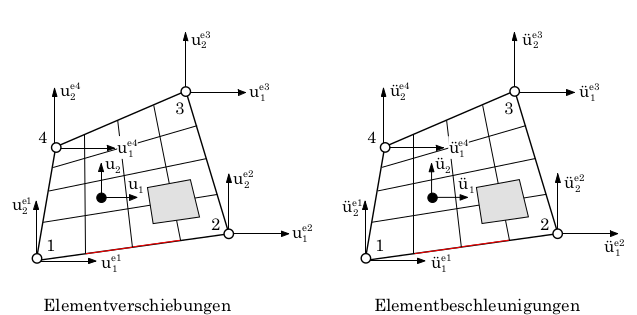
\includegraphics[scale=0.5]{Figure2/Chap2/4nodefredome.png}
    \caption{Degrees of freedom of a four-noded plane Lagrange element}
    \label{fig:3.11}
\end{figure}

Within the scope of the isoparametric element concept we can approximate the continuous
displacements, variation and second time derivative of displacements for $NN = 4$, analogous
with the approximation of the position vector in equation (\ref{eqn:341}) (see figure \ref{fig:3.11}).

\begin{equation}
 \begin{aligned} 
 \boldsymbol{u}(\boldsymbol{\xi}) & \approx \tilde{\boldsymbol{u}}(\boldsymbol{\xi})=\mathbf{N}(\boldsymbol{\xi}) \boldsymbol{u}^{e} & \boldsymbol{u}^{e} &=\left[\begin{array}
 {lllll}u_{1}^{e 1} & u_{2}^{e 1} & \cdots & u_{1}^{e N \mathrm{~N}} & u_{2}^{e N \mathbb{N}}
 \end{array}\right]^{T} \\ 
 \delta \boldsymbol{u}(\boldsymbol{\xi}) & \approx \delta \tilde{\boldsymbol{u}}(\boldsymbol{\xi})=\mathbf{N}(\boldsymbol{\xi}) \delta \boldsymbol{u}^{e} & \delta \boldsymbol{u}^{e} &= \left[
 \begin{array}{lllll}
     \delta u_{1}^{e 1}& \delta u_{2}^{e 1} &\cdots &\delta u_{1}^{e NN} &\delta u_{2}^{e N N}
 \end{array}
\right]^{T}   \\ 
 \ddot{\boldsymbol{u}}(\boldsymbol{\xi}) & \approx \tilde{\tilde{\boldsymbol{u}}}(\boldsymbol{\xi})=\mathbf{N}(\boldsymbol{\xi}) \ddot{\boldsymbol{u}}^{e} & \ddot{\boldsymbol{u}}^{e}
 &=\left[\begin{array}{lllll}\ddot{u}_{1}^{e 1} & \ddot{u}_{2}^{e 1} & \cdots & \ddot{u}_{1}^{e NN} & \ddot{u}_{2}^{e NN}\end{array}\right]^{T} 
 \end{aligned} 
 \label{eqn:3.59} 
\end{equation}

\subsection{Strain vector approximation}
To formulate the internal virtual work, the approximation of which is given with the help of
shape polynomials applied to displacements, and thereupon following integration of stiffness
terms, the strain vector components ought to be described in natural coordinates. This is ac-
complished by applying the derivation rule (\ref{eqn:3.51}) to the displacement strain relation in equation
\begin{equation}
\label{eqn:3.60} 
 \left[\begin{array}{c}\varepsilon_{11} \\ \varepsilon_{22} \\ 2 \varepsilon_{12}\end{array}\right]=\underbrace{\left[\begin{array}{ccc}\frac{\partial \xi_{1}}{\partial X_{1}} \frac{\partial}{\partial \xi_{1}}+\frac{\partial \xi_{2}}{\partial X_{1}} \frac{\partial}{\partial \xi_{2}} & 0 & \\ 0 & \frac{\partial \xi_{1}}{\partial X_{2}} \frac{\partial}{\partial \xi_{1}}+\frac{\partial \xi_{2}}{\partial X_{2}} \frac{\partial}{\partial \xi_{2}} \\ \frac{\partial \xi_{1}}{\partial X_{2}} \frac{\partial}{\partial \xi_{1}}+\frac{\partial \xi_{2}}{\partial X_{2}} \frac{\partial}{\partial \xi_{2}} & \frac{\partial \xi_{1}}{\partial X_{1}} \frac{\partial}{\partial \xi_{1}}+\frac{\partial \xi_{2}}{\partial X_{1}} \frac{\partial}{\partial \xi_{2}}\end{array}\right]}_{\mathbf{D}_{\varepsilon \xi}}\left[\begin{array}{c}u_{1} \\ u_{2}\end{array}\right], \quad \varepsilon=\mathbf{D}_{\varepsilon \xi} u 
\end{equation}

With the approximation of continuous displacements according to equation (\ref{eqn:3.59}), we get the
approximation of the strain vector from equation (\ref{eqn:3.60})
\begin{equation}
 \varepsilon(\boldsymbol{\xi}) \approx \tilde{\varepsilon}(\boldsymbol{\xi})=\mathbf{D}_{\varepsilon \xi}(\boldsymbol{\xi}) \tilde{\boldsymbol{u}}(\boldsymbol{\xi})=\mathbf{D}_{\varepsilon \xi}(\boldsymbol{\xi}) \mathbf{N}(\boldsymbol{\xi}) \boldsymbol{u}^{e}=\mathbf{B}(\boldsymbol{\xi}) \boldsymbol{u}^{e} \label{eqn:3.61} 
\end{equation}
by means of linear mapping of the element displacement vector and the differential operator
definition $\boldsymbol{B(\xi)}$.
\begin{equation}
\label{eqn:3.62}
 \tilde{\varepsilon}(\boldsymbol{\xi})=\mathbf{B}(\boldsymbol{\xi}) \boldsymbol{u}^{e} \qquad \qquad \mathbf{B}(\boldsymbol{\xi})=\mathbf{D}_{\varepsilon \xi}(\boldsymbol{\xi}) \mathbf{N}(\boldsymbol{\xi}) 
\end{equation}

The differential operator $B(\xi)$ is here given by applying $D \varepsilon\xi (\xi)$ to the matrix of shape functions
$N(\xi)$. If the operator $D _{\varepsilon\xi} (\xi)$ is not applied to the entire matrix of shape functions but only to
the submatrices $N i (\xi)$, we obtain the $B$-operator $B i (\xi)$ assigned to the element node i instead
of $B-operator B(\xi)$,
\begin{equation}
 \mathbf{B}_{i}(\boldsymbol{\xi})=\mathbf{D}_{\varepsilon \xi}(\boldsymbol{\xi}) \mathbf{N}^{i}(\boldsymbol{\xi}) \qquad  \qquad \mathbf{B}=\left[\begin{array}{lll}\mathbf{B}_{1} & \cdots & \mathbf{B}_{N \mathbf{N}}\end{array}\right], N N=4 
 \label{eqn:3.63} 
\end{equation}
with the differential operators $B_i(\xi)$ being matrix of the shape functions.
\begin{equation}
 \mathbf{B}_{i}(\boldsymbol{\xi})=\left[\begin{array}{ccc}\frac{\partial \xi_{1}}{\partial X_{1}} \frac{\partial}{\partial \xi_{1}}+\frac{\partial \xi_{2}}{\partial X_{1}} \frac{\partial}{\partial \xi_{2}} & 0 & \\ 0 & & \frac{\partial \xi_{1}}{\partial X_{2}} \frac{\partial}{\partial \xi_{1}}+\frac{\partial \xi_{2}}{\partial X_{2}} & \frac{\partial}{\partial \xi_{2}} \\ \frac{\partial \xi_{1}}{\partial X_{2}} \frac{\partial}{\partial \xi_{1}}+\frac{\partial \xi_{2}}{\partial X_{2}} \frac{\partial}{\partial \xi_{2}} & \frac{\partial \xi_{1}}{\partial X_{1}} \frac{\partial}{\partial \xi_{1}}+\frac{\partial \xi_{2}}{\partial X_{1}} & \frac{\partial}{\partial \xi_{2}}\end{array}\right]\left[\begin{array}{cc}N^{i}(\boldsymbol{\xi}) & 0 \\ 0 & N^{i}(\boldsymbol{\xi})\end{array}\right] 
 \label{eqn:3.64} 
\end{equation}

Finally, by applying the derivation rules we arrive at the portion of B-operator for element
node $i$.
\begin{equation}
 \mathbf{B}_{i}(\boldsymbol{\xi})=\left[\begin{array}{cc}\frac{\partial \xi_{1}}{\partial X_{1}} N_{; 1}^{i}(\boldsymbol{\xi})+\frac{\partial \xi_{2}}{\partial X_{1}} N_{; 2}^{i}(\boldsymbol{\xi}) & 0 \\ 0 & \frac{\partial \xi_{1}}{\partial X_{2}} N_{; 1}^{i}(\boldsymbol{\xi})+\frac{\partial \xi_{2}}{\partial X_{2}} N_{; 2}^{i}(\boldsymbol{\xi}) \\ \frac{\partial \xi_{1}}{\partial X_{2}} N_{; 1}^{i}(\boldsymbol{\xi})+\frac{\partial \xi_{2}}{\partial X_{2}} N_{; 2}^{i}(\boldsymbol{\xi}) & \frac{\partial \xi_{1}}{\partial X_{1}} N_{; 1}^{i}(\boldsymbol{\xi})+\frac{\partial \xi_{2}}{\partial X_{1}} N_{; 2}^{i}(\boldsymbol{\xi})\end{array}\right] 
 \label{eqn:3.65} 
\end{equation}


If the components of the inverse Jacobi matrix $\xi_{\alpha,\beta}$ according to equation (\ref{eqn:3.53}) are replaced by components of the Jacobi matrix $X_{\alpha,\beta}$ , it is possible to write down the $B$-operators $B_i (\xi)$ in the following way:
\begin{equation}
 \mathbf{B}_{i}(\boldsymbol{\xi})=\frac{1}{|\mathbf{J}(\boldsymbol{\xi})|}\left[\begin{array}{cc}\frac{\partial X_{2}}{\partial \xi_{2}} N_{; 1}^{i}(\boldsymbol{\xi})-\frac{\partial X_{2}}{\partial \xi_{1}} N_{; 2}^{i}(\boldsymbol{\xi}) & 0 \\ 0 & -\frac{\partial X_{1}}{\partial \xi_{2}} N_{; 1}^{i}(\boldsymbol{\xi})+\frac{\partial X_{1}}{\partial \xi_{1}} N_{; 2}^{i}(\boldsymbol{\xi}) \\ -\frac{\partial X_{1}}{\partial \xi_{2}} N_{; 1}^{i}(\boldsymbol{\xi})+\frac{\partial X_{1}}{\partial \xi_{1}} N_{; 2}^{i}(\boldsymbol{\xi}) & \frac{\partial X_{2}}{\partial \xi_{2}} N_{; 1}^{i}(\boldsymbol{\xi})-\frac{\partial X_{2}}{\partial \xi_{1}} N_{; 2}^{i}(\boldsymbol{\xi})\end{array}\right] 
 \label{eqn:3.66} 
\end{equation}

Derived in such a way, the B-operators contain matrix terms of the form $X _{\beta,\alpha} $ which again can be described as functions of shape function derivatives $N_{;a}^j(\xi)$ and of element node coordinates $X^{ij}_\beta$ according to equation (\ref{eqn:3.50}).
\begin{equation}
 \frac{\partial X_{\beta}}{\partial \xi_{\alpha}}=\frac{\partial}{\partial \xi_{\alpha}} \sum_{j=1}^{4} X_{\beta}^{e j} N^{j}(\boldsymbol{\xi})=\sum_{j=1}^{4} X_{\beta}^{e j} N_{; \alpha}^{j}(\boldsymbol{\xi}) 
 \label{eqn:3.67} 
\end{equation}
%--------------------------------------------------------------
\subsection{Appproximation of internal virtual work}

The internal virtual work is developed by substituting the stress vector by material law , by modifying the surface element $dA$ and by adjusting the integration
boundaries to natural coordinates $\xi_\alpha \in [{- 1}, 1]$.
\begin{equation}
 \delta W_{\mathrm{int}}^{e}=\int_{-1}^{1} \int_{-1}^{1} \delta \varepsilon(\boldsymbol{\xi}) \cdot \mathbf{C} \varepsilon(\boldsymbol{\xi})|\mathbf{J}(\boldsymbol{\xi})| h d \xi_{1} d \xi_{2} 
 \label{eqn:3.68} 
\end{equation}

Approximation of internal virtual work comes from substitution of the exact strain vector by
the approximated strain vector in equation (\ref{eqn:3.62})
\begin{equation}
 \delta \tilde{W}_{\mathrm{int}}^{e}=\int_{-1-1}^{1} \int_{-1}^{1} \delta \boldsymbol{u}^{e} \cdot \mathbf{B}^{T}(\boldsymbol{\xi}) \mathbf{C} \mathbf{B}(\boldsymbol{\xi}) \boldsymbol{u}^{e}|\mathbf{J}(\boldsymbol{\xi})| h d \xi_{1} d \xi_{2} 
 \label{eqn:3.69} 
\end{equation}

Due to the independence of the natural coordinates $\xi$ of both element displacement vectors $u^e$
and its variation $\epsilon u^e$ , both of these vectors can be exerted from the integral.

\begin{equation}
 \delta \tilde{W}_{\text {int }}^{e}=\delta \boldsymbol{u}^{e} \cdot \int_{-1}^{1} \int_{-1}^{1} \mathbf{B}^{T}(\boldsymbol{\xi}) \mathbf{C} \mathbf{B}(\boldsymbol{\xi})|\mathbf{J}(\boldsymbol{\xi})| h d \xi_{1} d \xi_{2} \boldsymbol{u}^{e}=\delta \boldsymbol{u}^{e} \cdot \mathbf{k}^{e} \boldsymbol{u}^{e} 
\label{eqn:3.70} 
\end{equation}

Here, we have defined the element stiffness matrix of a bilinear plane quadrangular element of
an arbitrary shape.
\begin{equation}
 \mathbf{k}^{e}=\int_{-1}^{1} \int_{-1}^{1} \mathbf{B}^{T}(\boldsymbol{\xi}) \mathbf{C} \mathbf{B}(\boldsymbol{\xi})|\mathbf{J}(\boldsymbol{\xi})| h d \xi_{1} d \xi_{2} 
\label{eqn:3.71} 
\end{equation}

The element thickness can be independent of the location in case of a plane stress state
$(h = h(\xi))$ ; in case of a plane strain state, the element thickness is constant. It is customary to add the integrand which is evaluated and weighed at the Gauss
points and formed with the help of the $B$-operator, the Jacobi determinant and the element
thickness, to the element stiffness matrix. The so called full integration or the $2 x 2$ integration
of a bilinear element accordingly requires four calculations of an integrand and its weighed
addition.
\begin{equation}
 \mathbf{k}^{e} \approx \sum_{i=1}^{2} \sum_{j=1}^{2} \alpha^{i} \alpha^{j} \mathbf{B}^{T}\left(\xi_{1}^{i}, \xi_{2}^{j}\right) \mathbf{C} \mathbf{B}\left(\xi_{1}^{i}, \xi_{2}^{j}\right)\left|\mathbf{J}\left(\xi_{1}^{i}, \xi_{2}^{j}\right)\right| h\left(\xi_{1}^{i}, \xi_{2}^{j}\right) 
 \label{eqn:3.72} 
\end{equation}

Gauss points $\xi_\alpha^i$ and weighting factors $\alpha^i$ of numeric integration can be found in figure \ref{fig:222}. Apart from the full integration, a subintegration of the bilinear element is also introduced with only
one Gauss point in the midpoint of the element. Merely in special cases of element geometry, it
is reasonable to determine the element stiffness by analytical derivation of the $B$-operator and analytical integration. 

\subsection{Approximation of dynamic virtual work}

Besides discretization of internal virtual work, transient mechanical problems also demand discretization of dynamic virtual work. If we, in the principle of virtual displacements, replace the surface element $dA$ and the integration boundaries 
\begin{equation}
 \delta W_{\mathrm{dyn}}^{e}=\int_{-1-1}^{1} \int_{1}^{1} \delta \boldsymbol{u}(\boldsymbol{\xi}) \cdot \ddot{\boldsymbol{u}}(\boldsymbol{\xi})|\mathbf{J}(\boldsymbol{\xi})| \rho h d \xi_{1} d \xi_{2} 
 \label{eqn:3.73} 
\end{equation}
and if we approximate the variation of displacements as well as continuous accelerations with
the assistance of shape functions according to equation (\ref{eqn:3.59}), we get the approximation of
virtual work of inertial forces.
\begin{equation}
 \delta \tilde{W}_{\mathrm{dyn}}^{e}=\delta \boldsymbol{u}^{e} \cdot \int_{-1-1}^{1} \int_{-1}^{1} \mathbf{N}^{T}(\boldsymbol{\xi}) \mathbf{N}(\boldsymbol{\xi})|\mathbf{J}(\boldsymbol{\xi})| \rho h d \xi_{1} d \xi_{2} \ddot{\boldsymbol{u}}^{e}=\delta \boldsymbol{u}^{e} \cdot \mathbf{m}^{e} \ddot{\boldsymbol{u}}^{e} 
 \label{eqn:3.74} 
\end{equation}

For purposes of defining the element mass matrix, we repeatedly took advantage of the fact
that the element vectors $\varepsilon u^e$ and $\ddot{o}^e$ are independent of natural coordinates.
\begin{equation}
 \mathbf{m}^{e}=\int_{-1}^{1} \int_{-1}^{1} \mathbf{N}^{T}(\boldsymbol{\xi}) \mathbf{N}(\boldsymbol{\xi})|\mathbf{J}(\boldsymbol{\xi})| \rho h d \xi_{1} d \xi_{2} 
\label{eqn:3.75} 
\end{equation}
\subsection{Approximation of virtual work of external loads}

The loads acting on a plane element can be divided into loads acting in the field and those acting at the boundaries of the field. Typical loads in the field are gravitational loads whereas actual structural loads are dominated by boundary loads such as pressure.

\vspace{0.38cm} \textbf{a) \textit{Volume loads}} \\

With the help of displacement variation approximation as in equation (\ref{eqn:3.59}), a consistent element load vector of volume loads $b(\xi)$ can be obtained based on external virtual work.
\begin{equation}
 \delta \tilde{W}_{\mathrm{ext}}^{\Omega e}=\delta \boldsymbol{u}^{e} \cdot \int_{-1}^{1} \int_{-1}^{1} \mathbf{N}^{T}(\boldsymbol{\xi}) \boldsymbol{b}(\boldsymbol{\xi})|\mathbf{J}(\boldsymbol{\xi})| \rho h d \xi_{1} d \xi_{2}=\delta \boldsymbol{u}^{e} \cdot \boldsymbol{r}_{p}^{e} 
\label{eqn:3.76} 
\end{equation}

Element vector of volume forces:

\begin{equation}
 \boldsymbol{r}_{p}^{e}=\int_{-1}^{1} \int_{-1}^{1} \mathbf{N}^{T}(\boldsymbol{\xi}) \boldsymbol{b}(\boldsymbol{\xi})|\mathbf{J}(\boldsymbol{\xi})| \rho h d \xi_{1} d \xi_{2} 
 \label{eqn:3.77} 
\end{equation}

Usually, $b$ is not given as dependent of natural coordinates $\xi$ but as function of physical
coordinates X. In such a case, the position of volume load has to be transformed to natural
coordinates $( b(X) \rightarrow b(\xi))$.

\vspace{0.38cm} \textbf{b) \textit{Boundary loads}} \\

The element load vector of element boundary loads $\boldsymbol{t*(\xi)}h$ is derived by observation of external virtual work . Here, the boundary $\Gamma$ σ can here be divided into four
boundaries $\Gamma_i$ i of the element.
\begin{equation}
 \delta W_{\mathrm{ext}}^{\Gamma e}=\int_{\Gamma_{\sigma}} \delta \boldsymbol{u} \cdot \boldsymbol{t}^{\star} h d \Gamma_{\sigma}=\sum_{i=1}^{4} \int_{\Gamma_{i}} \delta \boldsymbol{u} \cdot \boldsymbol{t}^{\star} h d \Gamma_{i}=\sum_{i=1}^{4} \delta W_{\mathrm{ext}}^{\Gamma_{i} e} 
 \label{eqn:3.78} 
\end{equation}

As an example, the proceeding for calculating the consistent equivalent loads is demonstrated
for element boundary three that connects nodes three and four. As shown in figure \ref{eqn:3.12}, the element edge is characterised by the natural coordinate $\xi_2 = 1$.

\begin{equation}
 \delta W_{\mathrm{ext}}^{\Gamma_{3 e}}=\int_{\Gamma_{3}} \delta \boldsymbol{u}\left(\xi_{1}, 1\right) \cdot \boldsymbol{t}^{\star}\left(\xi_{1}, 1\right) h d \Gamma_{3} 
 \label{eqn:3.79} 
\end{equation}

To integrate this integrand over element edge three, the line element $d\gamma_3$ must be transformed
into the natural coordinate $d\xi_1$ . The differential line element here is analysed in physical space. Projection of line element $d\gamma_3$ onto direction $e_1$ yields the differential physical line element $dX_ 1$ , projection onto direction $e_ 2$ yields $dX_2$ . Vice versa, the square of line element can be calculated with the Pythagoras theorem.
\begin{equation}
 d \Gamma_{3}^{2}=d X_{1}^{2}+d X_{2}^{2} 
 \label{eqn:3.80} 
\end{equation}
\begin{figure}
    \centering
    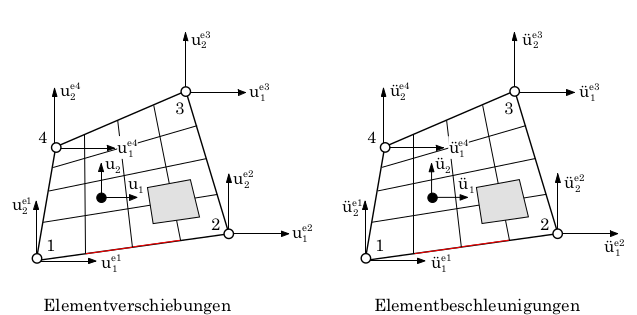
\includegraphics[scale=0.5]{Figure2/Chap2/4nodefredome.png}
    \caption{External loads of a four-noded Lagrange element}
    \label{fig:my_label}
\end{figure}

The total differentials $dX_\beta$ for $ \beta = 1, 2$ are found to be functions of total differentials in natural
coordinates and in Jacobi matrix components. It should be noted here that the differential $d\xi_2$
vanishes $(d\xi _2 = 0) $ at element edge three$ (\xi_ 2 = 1)$.
\begin{equation}
 d X_{\beta}=\frac{\partial X_{\beta}}{\partial \xi_{1}} d \xi_{1}+\frac{\partial X_{\beta}}{\partial \xi_{2}} d \xi_{2}=\frac{\partial X_{\beta}}{\partial \xi_{1}} d \xi_{1} 
\label{eqn:3.81}
\end{equation}

Inserting equation (\ref{eqn:3.81}) into equation (\ref{eqn:3.80}) yields the transformation relation of line element
$d\Gamma_3$ .

\begin{equation}
 d \Gamma_{3}^{2}=\left[\left(\frac{\partial X_{1}}{\partial \xi_{1}}\right)^{2}+\left(\frac{\partial X_{2}}{\partial \xi_{1}}\right)^{2}\right] d \xi_{1}^{2} 
 \label{eqn:3.82} 
\end{equation}

If we additionally introduce the Jacobi determinant$|J_3 (\xi_ 1 , 1)|$, which generally is a function of coordinate $\xi_1$ , we can write down the transformation relation (\ref{eqn:3.82}) in a familiar compact
form.
\begin{equation}
 d \Gamma_{3}=\left|\mathbf{J}_{3}\left(\xi_{1}, 1\right)\right| d \xi_{1} \quad\left|\mathbf{J}_{3}\left(\xi_{1}, 1\right)\right|=\left[\left(\frac{\partial X_{1}}{\partial \xi_{1}}\right)^{2}+\left(\frac{\partial X_{2}}{\partial \xi_{1}}\right)^{2}\right]^{\frac{1}{2}} 
 \label{eqn:3.83} 
\end{equation}

Formally, the same transformation relation is found for line element $d\Gamma_ 1$ , where the partial
derivatives in equation (3.81) must be evaluated for natural coordinate $\xi_ 2 = −1$ instead of
$\xi_ 2 = 1$. Analogous observations lead to transformation relation of line elements $d\Gamma_ 2$ and $d\Gamma_ 4$ .
Transformation of the line element $d\Gamma_ 4$ is given which is valid for both line elements.

\begin{equation}
 d \Gamma_{3}=\left|\mathbf{J}_{3}\left(\xi_{1}, 1\right)\right| d \xi_{1} \qquad \left|\mathbf{J}_{3}\left(\xi_{1}, 1\right)\right|=\left[\left(\frac{\partial X_{1}}{\partial \xi_{1}}\right)^{2}+\left(\frac{\partial X_{2}}{\partial \xi_{1}}\right)^{2}\right]^{\frac{1}{2}} 
 \label{eqn:3.84} 
\end{equation}
Back to element edge three and the boundary load of bilinear Lagrange elements. Next, the
position vector on the element edge according to equation (\ref{eqn:339}) is described with the help
of shape functions $N_ i (\xi_ 1 , 1), i = 1, 2, 3, 4 $, as a basis of transformation (\ref{eqn:3.83}). A reduction
of shape functions is not necessary here since the shape functions corresponding to element
nodes one and two vanish at the element edge three ($N_1 (\xi 1 , 1) = N_2 (\xi 1 , 1) = 0$, see equation
(\ref{eqn:3.35}) 
\begin{equation}
 \boldsymbol{X}\left(\xi_{1}, 1\right)=\sum_{i=1}^{4} \boldsymbol{X}^{e i} N^{i}\left(\xi_{1}, 1\right)=\sum_{i=3}^{4} \boldsymbol{X}^{e i} N^{i}\left(\xi_{1}, 1\right) 
 \label{eqn:3.85} 
\end{equation}

Derivative of the position vector with respect to natural coordinate $\xi_1$ is given by
\begin{equation}
 \frac{\partial \boldsymbol{X}\left(\xi_{1}, 1\right)}{\partial \xi_{1}}=\sum_{i=1}^{4} \boldsymbol{X}^{e i} N_{; 1}^{i}\left(\xi_{1}, 1\right)=\mathbf{N}_{; 1}\left(\xi_{1}, 1\right) \boldsymbol{X}^{e} 
 \label{eqn:3.86} 
\end{equation}
and the derivative with respect to $\xi_2$ is zero. Horizontal and vertical components $dX \beta , \beta = 1, 2$
of line element $ d\Gamma _3 $are found by calculation of total differentials according to equation (\ref{eqn:3.36}),
where derivatives of shape functions according to equation (\ref{eqn:3.81}) are directly used for $\xi_2 = 1$.
\begin{equation}
 d X_{\beta}=\frac{\partial X_{\beta}\left(\xi_{1}, 1\right)}{\partial \xi_{1}} d \xi_{1}=\left[X_{\beta}^{e 3} N_{; 1}^{3}\left(\xi_{1}, 1\right)+X_{\beta}^{e 4} N_{; 1}^{4}\left(\xi_{1}, 1\right)\right] d \xi_{1}=\left[X_{\beta}^{e 3} \frac{1}{2}-X_{\beta}^{e 4} \frac{1}{2}\right] d \xi_{1} 
 \label{eqn:3.87} 
\end{equation}

With equation (\ref{eqn:3.83}), the sought Jacobi determinant $|J_3 (\xi_ 1 , 1)|$ of a bilinear Lagrange element
finally follows, related to element edge three.
\begin{equation}
 \begin{aligned}\left|\mathbf{J}_{3}\left(\xi_{1}, 1\right)\right| &=\left[\left(X_{1}^{e 3} \frac{1}{2}-X_{1}^{e 4} \frac{1}{2}\right)^{2}+\left(X_{2}^{e 3} \frac{1}{2}-X_{2}^{e 4} \frac{1}{2}\right)^{2}\right]^{\frac{1}{2}} \\ &=\frac{1}{2}\left[\left(X_{1}^{e 3}-X_{1}^{e 4}\right)^{2}+\left(X_{2}^{e 3}-X_{2}^{e 4}\right)^{2}\right]^{\frac{1}{2}} \end{aligned}
 \label{eqn:3.88} 
\end{equation}

With this we can substitute the line element dΓ 3 in equation (\ref{eqn:3.79}) as well as the integration
boundaries by a differential of the natural coordinate $\xi_1 $ that is by interval boundaries of the
natural coordinate $\xi_1 \in [−1, 1]$.
\begin{equation}
 \delta W_{\mathrm{ext}}^{\Gamma_{3}}=\int_{-1}^{1} \delta \boldsymbol{u}\left(\xi_{1}, 1\right) \cdot \boldsymbol{t}^{\star}\left(\xi_{1}, 1\right) h\left|\mathbf{J}_{3}\left(\xi_{1}, 1\right)\right| d \xi_{1} 
 \label{eqn:3.89} 
\end{equation}

The approximation of displacement variation according to equation (\ref{eqn:3.59})
\begin{equation}
 \delta \tilde{W}_{\mathrm{ext}}^{\Gamma_{3}}=\delta \boldsymbol{u}^{e} \cdot \int_{-1}^{1} \mathbf{N}^{T}\left(\xi_{1}, 1\right) \boldsymbol{t}^{\star}\left(\xi_{1}, 1\right) h\left|\mathbf{J}_{3}\left(\xi_{1}, 1\right)\right| d \xi_{1}=\delta \boldsymbol{u}^{e} \cdot \boldsymbol{r}_{n 3}^{e} 
 \label{eqn:3.90} 
\end{equation}
finally yields the consistent equivalent load of the boundary load $r^e_{n3}$ .
\begin{equation}
 \boldsymbol{r}_{n 3}^{e}=\int_{-1}^{1} \mathbf{N}^{T}\left(\xi_{1}, 1\right) \boldsymbol{t}^{\star}\left(\xi_{1}, 1\right) h\left|\mathbf{J}_{3}\left(\xi_{1}, 1\right)\right| d \xi_{1} 
 \label{eqn:3.91} 
\end{equation}

The summation of all correspondingly calculated equivalent loads $r_{ni}$ for $i = 1, 2, 3, 4$ yields the
consistent equivalent loads of an element.
\begin{equation}
 \delta \tilde{W}_{\mathrm{ext}}^{\Gamma}=\sum_{i=1}^{4} \delta \tilde{W}_{\mathrm{ext}}^{\Gamma_{i}}=\sum_{i=1}^{4} \delta \boldsymbol{u}^{e} \cdot \boldsymbol{r}_{n i}^{e}=\delta \boldsymbol{u}^{e} \cdot \sum_{i=1}^{4} \boldsymbol{r}_{n i}^{e}=\delta \boldsymbol{u}^{e} \cdot \boldsymbol{r}_{n}^{e} 
 \label{eqn:3.92} 
\end{equation}

The integration of consistent equivalent loads according to equation (3.91) is performed mostly
numerically, too. As opposed to integration of $k _e , m_ e $or $r _{ep} $, one-dimensional numerical integration is necessary here. 
It may be noted here that virtual works of boundary loads of adjacent elements cancel each
other out. For this reason, it is sufficient to calculate the virtual works of boundary loads at free
boundaries that are not only element boundaries but also represent system boundaries.